\chapter{背景知识}

% Sec 2.1
\section{LBM的起源}
格子玻尔兹曼方法起源于格子气自动机 (lattice gas automata, LGA) 方法。如方法中的名字所述,LBM继承了方法中格子的概念。LGA依赖于微观方法,在该方法中流体系统使用粒子描述,而非我们一般接触的宏观连续状态量。这些粒子在计算中并不能自由地无规则运动,而有一定的约束。在一个规则网格中,这些粒子只会在网格的相邻节点间\textit{迁移},并在格点发生\textit{碰撞}。在真实世界中,每次碰撞后粒子的速度应该是一个连续的独立变量,并可以先验得到。而因为格子的存在,速度空间只能被离散化,而不再是连续的空间。在一类LGA中,格子可能是六边形的,如图~\ref{img:LGA_lattice}所示,该类方法被称为FHP方法~\cite{frisch1986lattice},该方法根据三位提出者Frisch、Hasslacher与Pomeau命名。

\begin{figure}[htb]
    \centering
      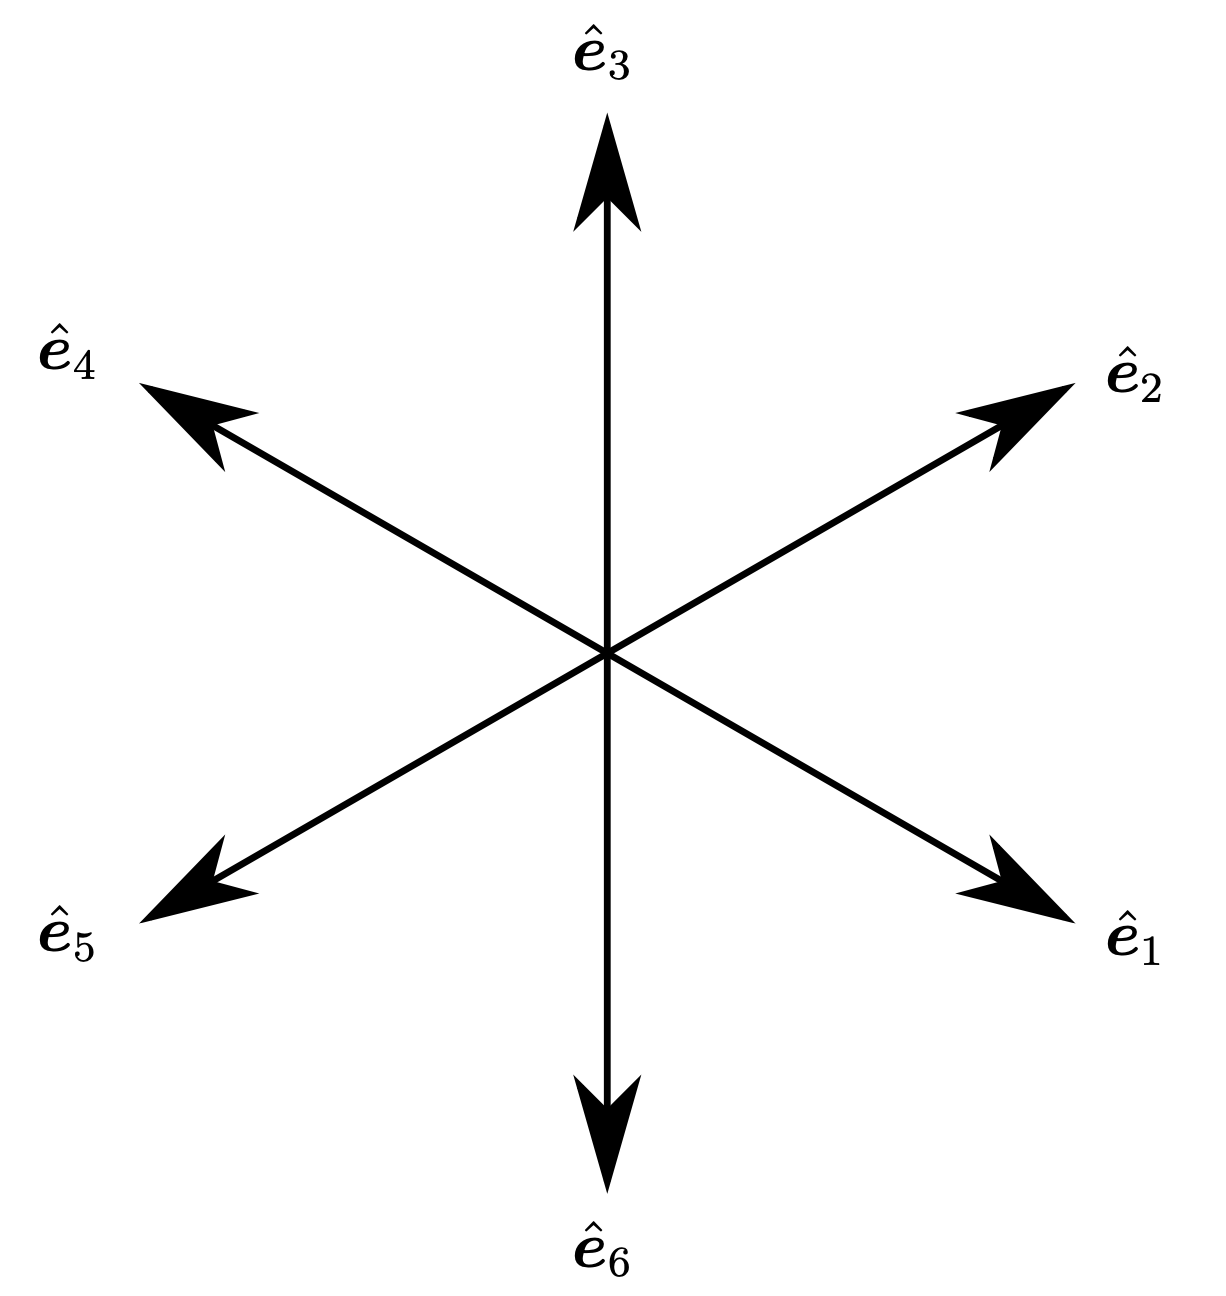
\includegraphics[width=0.5\columnwidth]{figures/LGA_lattice.png}
    \bicaption{\TODO{XXX}}{Hexagonial lattice of the FHP model with six discrete velocity directions in two-dimensional velocity space.}
    \label{img:LGA_lattice}
\end{figure}

不论LGA或LBM,有一个通用的假设是,在一个时间步长$\Delta t$后,一个粒子会正好走过两个相邻格点间的距离$\Delta x$。对于一个六边形网格,有
\begin{equation}
    \mathbf{\xi}_i=\frac{\Delta x}{\Delta t}\hat{\mathbf{e}}_i,
\end{equation}
其中$\hat{\mathbf{e}}_i=\mathbf{e}_i/|\mathbf{e}_i|$是正则化后的粒子运动方向,$i$是速度方向的标号,$\mathbf{\xi}_i$是离散速度。那么接下来可以定义粒子的状态$n_{i}(\mathbf{x},t)$,这个状态值可以是0或1。不考虑碰撞的话,粒子的运动可以用方程描述:
\begin{equation}
    n_{i}(\mathbf{x}+\mathbf{\xi}_i \Delta t,t+\Delta t)=n_{i}(\mathbf{x},t).
    \label{eq:LGA}
\end{equation}
公式~\ref{eq:LGA}构成了LGA中标志性的迁移步骤。这一过程也被LBM所继承。这一点为LBM方法带来了很大的优势,首先就是线性的对流项大幅降低了计算难度。其次是这一种直接的空间离散形式并不需要生成一个特殊的计算网格,使前处理的复杂度也能大幅下降。然而这并不代表LBM对网格完全没有要求,这类基于格子的方法只能被应用于六边形或更常见的笛卡尔网格也是一种对网格的约束。

在LGA中,因为粒子只有两种状态,所以经常使用布尔 (Boolean) 变量表示。一般值为真 (true) 时表示在某个空间位置上有一个粒子正在以特定的速度移动,而值为假 (false) 时表示没有这样的粒子。这清楚地显示LGA方法是在粒子层面来表示流体的运动的~\cite{wolf2004lattice}。而很显然,想要完全真实地使用粒子来表示流体是不现实的,因为$1cm^3$的空气中就含有约$2.7\times 10^{19}$个粒子。这导致LGA只能采用比现实情况要低得多的粒子量进行仿真,使结果有很强的噪声。从而方法需要在空间和时间上进行平均才能取得相对正常的结果。为了解决这一问题,McNamara和Zanetti~(\citeyear{mcnamara1988use})提出使用一个表示粒子密度的分布函数来替代这种单个的粒子。这种抽象的表达也是玻尔兹曼输运方程 (Boltzmann Transport Equation, BTE) 的构成基础。所以被传输的值不再只是一个布尔值,而是一个实数。这个实数表达了在空间位置$\mathbf{x}$、时间$t$,找到一个速度为$\mathbf{\xi}$的粒子的概率的空间密度。那么在没有碰撞时的迁移步骤的方程变为:
\begin{equation}
    f_{i}(\mathbf{x}+\mathbf{\xi}_i \Delta t,t+\Delta t)=f_{i}(\mathbf{x},t),
    \label{eq:LBM_streaming}
\end{equation}
其中$f_{i}$是上述的概率分布函数,一般简称为分布函数。一般认为这标志着LBM的诞生。因为在微观过程上使用了统计的概念,所以LBM被称为介观 (mesoscopic) 方法。在公式~\ref{eq:LGA}与~\ref{eq:LBM_streaming}中,粒子间的交互被忽略了。考虑粒子间的交互,这个过程可以表示为
\begin{equation}
    f_{i}(\mathbf{x}+\mathbf{\xi}_i \Delta t,t+\Delta t)=f_{i}(\mathbf{x},t)+\Omega(f_{i}(\mathbf{x},t)),
    \label{eq:LBM_in_one}
\end{equation}
其中$\Omega$是碰撞运算符。然而在实际中,通常会将公式~\ref{eq:LBM_in_one}表示为两个分开的过程,即碰撞和迁移:
\begin{alignat}{2}
\textbf{碰撞:} & \quad\quad &f_i^*(\boldsymbol{x}, t) & =f_i(\boldsymbol{x}, t)+\Omega\left(f_i(\boldsymbol{x}, t)\right); \\
\textbf{迁移:} & & f_i\left(\boldsymbol{x}+\boldsymbol{\xi}_i \Delta t, t+\Delta t\right) & =f_i^*(\boldsymbol{x}, t),
\end{alignat}
其中,$f_i^*$表示碰撞后的分布函数。为了满足质量与动量守恒,LGA中的碰撞中设定了一些固定的规则。对于FHP模型来说,其只允许两个或三个粒子间的碰撞,并且粒子离开格点的方向不能和进入格点的方向一样。这使得两个粒子间的碰撞只有两种可能的结果,而三个粒子间的碰撞只有一种可能的结果,参见图~\ref{img:LGA_collision}。

\begin{figure}[htb]
    \centering
      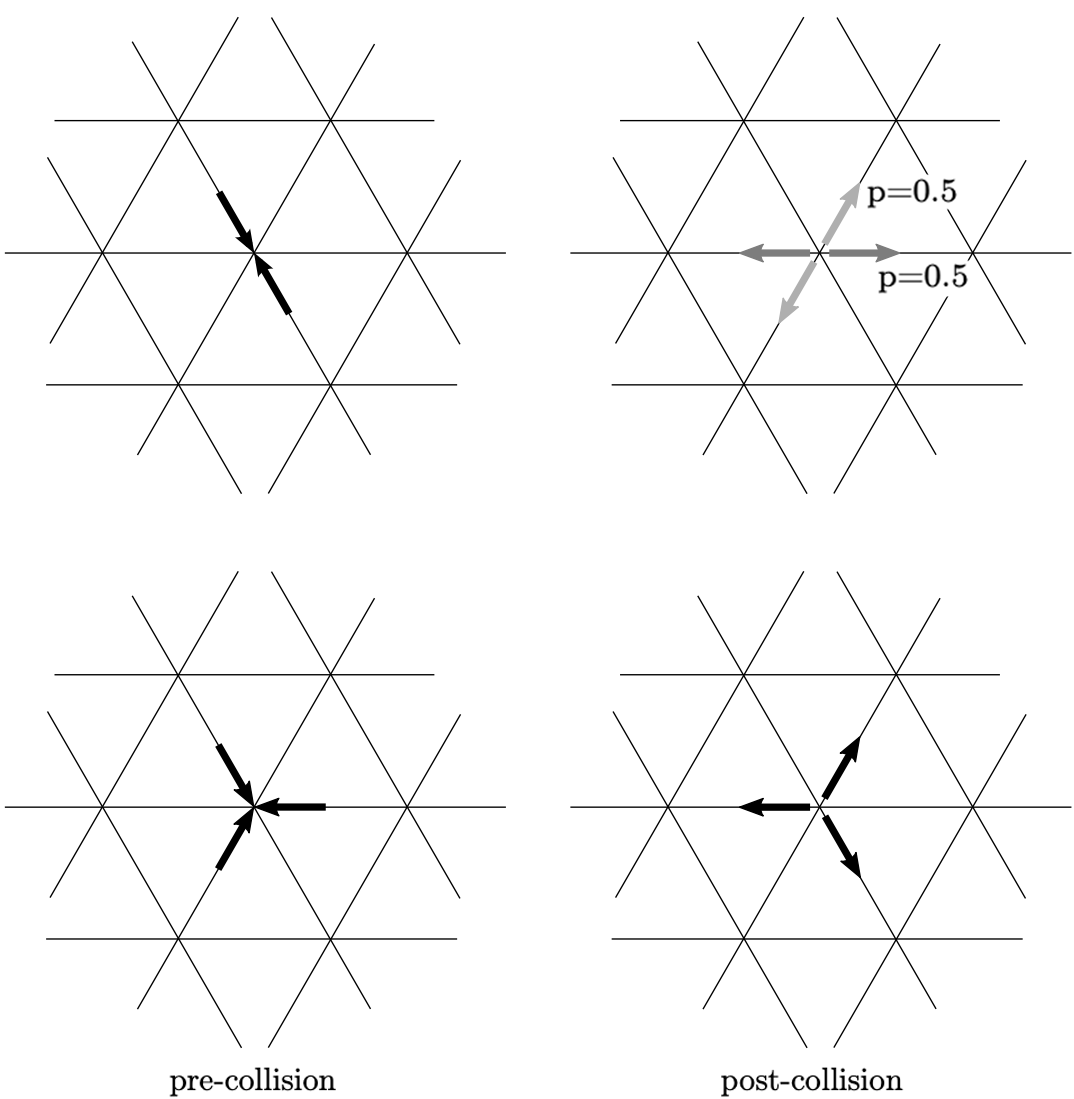
\includegraphics[width=0.9\columnwidth]{figures/LGA_collision.png}
    \bicaption{\TODO{XXX}}{Two- and three-particle collision in the FHP model. p denotes the probablility of a particular post-collision state.}
    \label{img:LGA_collision}
\end{figure}

虽然,最初的LB模型也是基于这些碰撞规则,但是很快人们发现这样的碰撞规则不仅物理上不够精确,对于三维来说,所需的计算量也是不现实的。于是另一种增强的碰撞方案被提出~\cite{higuera1989lattice, higuera1989boltzmann},该方案将非线性的碰撞运算进行了线性化,使碰撞后的值与一个平衡态产生联系:
\begin{equation}
    \Omega(f_{i}(\mathbf{x}, t))=\mathbf{A}_{\alpha\beta}(f_{i}(\mathbf{x},t)+f_{i}^{eq}(\mathbf{x},t)),
\end{equation}
其中$\mathbf{A}$是一个散射矩阵 (scattering matrix),$f_{i}^{eq}$是离散的麦克斯韦-玻尔兹曼平衡态函数 (Maxwell-Boltzmann equilibrium function)。之后Qian等~(\citeyear{qian1992lattice}) 进一步对碰撞模型的简化,基本确定了现在最常见的LBM的碰撞形式,即粒子间的碰撞可以看作是分布函数向平衡态的一个松弛过程:
\begin{equation}
    \mathbf{A}=-\delta_{\alpha\beta}\tilde{\omega}.
\end{equation}
那么这个散射矩阵事实上可以被一个松弛系数$\tilde{\omega}$替代了,这个系数是松弛时间$\tilde{\tau}$的倒数:$\tilde{\omega}^{-1}=\tilde{\tau}=\frac{\tau}{\Delta t}$. 从而,公式~\ref{eq:LBM_in_one}变为
\begin{equation}
    f_{i}(\mathbf{x}+\mathbf{\xi}_i \Delta t,t+\Delta t)=f_{i}(\mathbf{x},t)-\tilde{\omega}(f_{i}(\mathbf{x},t)-f_{i}^{eq}(\mathbf{x},t)).
    \label{eq:LBM_in_one_BGK}
\end{equation}
现在所有的分布函数都以相同的速率向平衡态松弛,虽然这样非常地简洁高效,但是这种方法没有考虑对于分布函数中有物理意义和没有意义的部分是否需要分开处理。之后d'Humières~(\citeyear{d1992generalized}) 证明散射矩阵$\mathbf{A}$可以由一组特征基得到,这为多松弛时间模型的出现奠定了基础。

这种对碰撞本身的效果建模,而不是对微观过程建模的想法,最早可见于连续玻尔兹曼方程中的BGK碰撞模型~\cite{Bhatnagar-1954}。这个想法背后的动机是碰撞过程的大部分细节并不会对宏观量产生影响,所以可以将这些过程省略。除了质量与动量守恒之外,BGK模型还满足$\mathrm{H}$-定理,即分布函数会向平衡态趋近。基于BGK的LBM也是最简洁、最常见的LBM模型。


% Sec 2.2
\section{从介观量到宏观量}
对于大多数的流体应用,使用一组连续的状态量来描述,如速度、压力等一般已经足够。这些量其实是微观粒子状态的统计平均。在宏观上,流体可以被视为连续体并由N-S方程描述。然而LBM并非是一个宏观方法,而是介于微观与宏观之间的介观层面,如图~\ref{img:fluid_abstraction}所示。

\begin{figure}[htb]
    \centering
      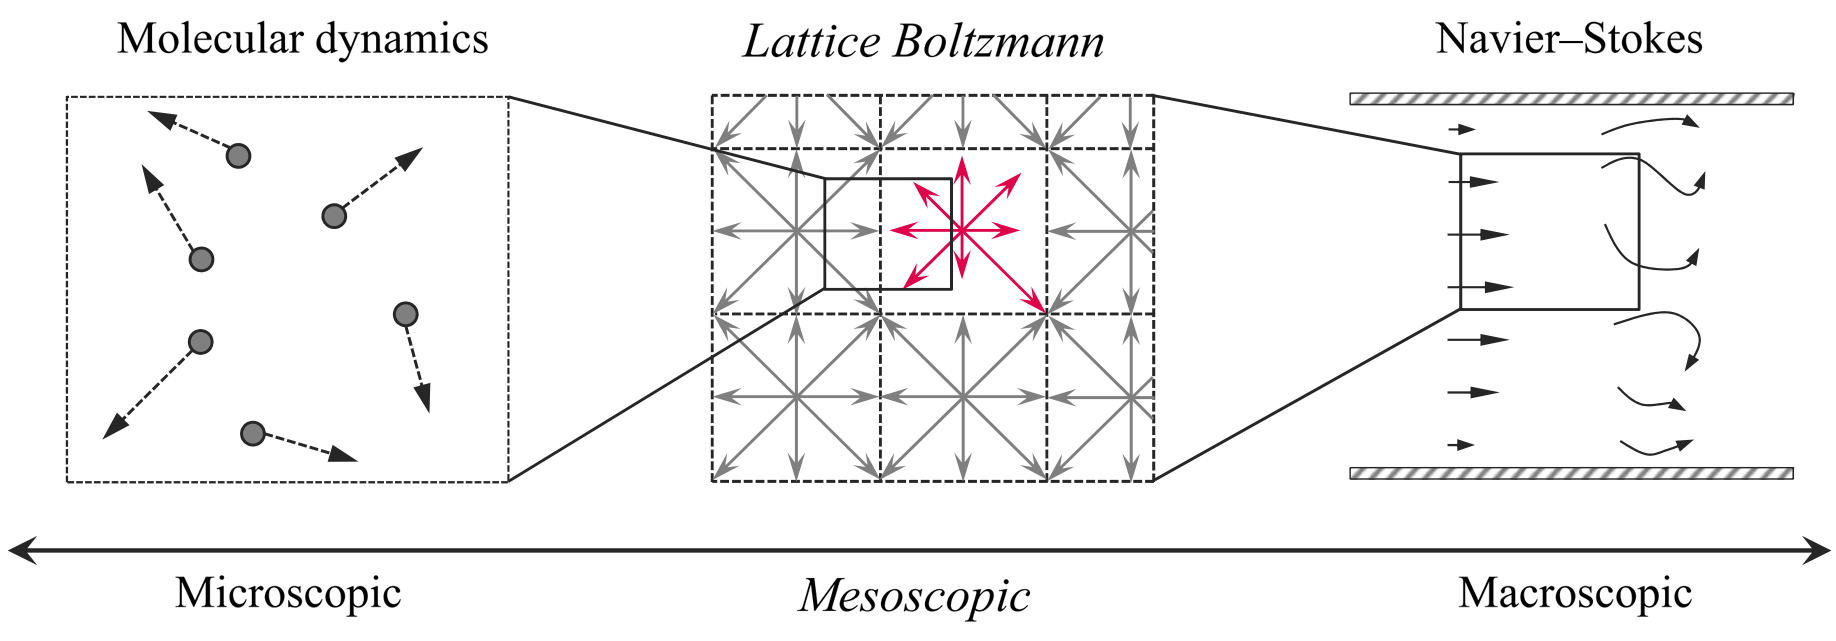
\includegraphics[width=0.9\columnwidth]{figures/fluid_abstraction.png}
    \bicaption{\TODO{XXX}}{Different abstraction levels of the fluid dynamics.}
    \label{img:fluid_abstraction}
\end{figure}

可以认为LBM虽然采用了一种非常简化的方案,但它依然计算了部分的微观层面的交互。这也使得LBM的求解过程与N-S方程求解有本质的区别。然而我们最终目的依然是获取宏观的流体状态,以符合我们在宏观世界中对流体的感受。接下来我们将逐步介绍LBM中的概念,并建立其与宏观世界的联系。

可以认为,在一个给定的控制体积 (control volume) 中,分布函数表示了速度在$\boldsymbol{Xi}$与$\boldsymbol{Xi}+d\boldsymbol{Xi}$之间的粒子总数。所以宏观和介观值可以通过对速度空间$\boldsymbol{Xi}$积分来建立,通过积分我们可以得到速度的n阶矩
\begin{equation}
    \boldsymbol{M}^{(n)}=\int_{\mathbb{R}^{\mathrm{D}}} \underbrace{\boldsymbol{\xi} \boldsymbol{\xi} \ldots \boldsymbol{\xi}}_{\mathrm{n} \text {次}} f(\boldsymbol{x}, \boldsymbol{\xi}, t) \mathrm{d} \boldsymbol{\xi},
\end{equation}
这里$D$代表积分的维度。在宏观层面,质量、动量和能量的守恒是由方程自身保证的,然而在介观层面,这些量的守恒需要由碰撞运算符保证,即
\begin{equation}
    \int\left(\Omega(f) \cdot \psi\right) \mathrm{d} \boldsymbol{\xi}=0,
    \label{eq:collision_invariants}
\end{equation}
其中$\psi_k$是碰撞不变量 (collision invariants),也就是可以令公式~\ref{eq:collision_invariants}成立的变量。可以证明,当$\psi=1, \boldsymbol{\xi}, |\boldsymbol{\xi}|^2$时,公式~\ref{eq:collision_invariants}是成立的。如果我们将碰撞不变量与分布函数的积进行积分,我们可以自然地得到连续速度空间中的宏观量
\begin{equation}
    \left\{\begin{array}{l}\rho(\boldsymbol{x}, t)=\int f(\boldsymbol{x}, \boldsymbol{\xi}, t) \mathrm{d} \boldsymbol{\xi} \\ \rho \boldsymbol{u}(\boldsymbol{x}, t)=\int \boldsymbol{\xi} f(\boldsymbol{x}, \boldsymbol{\xi}, t) \mathrm{d} \boldsymbol{\xi} \\ \rho E(\boldsymbol{x}, t)=\frac{1}{2} \int|\boldsymbol{\xi}|^2 f(\boldsymbol{x}, \boldsymbol{\xi}, t) \mathrm{d} \boldsymbol{\xi}\end{array}\right.,
\end{equation}
其中$E$为比能量 (specific energy)。对于单原子气体,碰撞可以假设为弹性的,所以比能量包含内能与动能
\begin{equation}
    \rho E=\rho\left(e+\frac{1}{2}|\boldsymbol{u}|^2\right).
\end{equation}
对于本动速度 (peculiar velocity) $\boldsymbol{v}=\boldsymbol{\xi}-\boldsymbol{u}$,即粒子在速度为$\boldsymbol{u}$的平均流中的相对速度,我们可以得到类似的能量守恒定律:
\begin{equation}
    \rho e(\boldsymbol{x}, t)=\frac{1}{2} \int|\boldsymbol{v}|^2 f(\boldsymbol{x}, \boldsymbol{\xi}, t) \mathrm{d} \boldsymbol{\xi}.
\end{equation}
在连续概念的流体力学中,内能的守恒方程需要通过一个状态方程$p=p(\rho,e)$将压力和密度联系起来,即
\begin{equation}
    p=\frac{1}{\mathrm{D}} \int|\boldsymbol{v}|^2 f(\boldsymbol{x}, \boldsymbol{\xi}, t) \mathrm{d} \boldsymbol{\xi}=\frac{2}{\mathrm{D}} \rho e.
    \label{eq:eos}
\end{equation}
对于满足理想气体定律 (perfect gas law) 的等温流体,可以得到
\begin{equation}
    e=\frac{\mathrm{D}}{2} \frac{p}{\rho}=\frac{\mathrm{D}}{2} R T_0=\frac{\mathrm{D}}{2} \frac{k_B T_0}{m}=\frac{\mathrm{D}}{2} c_s^2,
\end{equation}
其中$T_0$和$c_s$分别表示常值的温度与声速。所以公式~\ref{eq:eos}可以被重写为
\begin{equation}
    p=\rho c_s^2,
\end{equation}
即绝热系数$\gamma=1$时的等熵状态方程~\cite{kundu2015fluid}。


% Sec 2.3
\section{速度空间的离散化}
为了对速度空间进行离散,离散分布函数$f$对于任意阶的矩均有贡献,所以对于$f$,应该有一个多项式的表达。
